\section{Structure Learning}

\begin{frame}{Challenges in Structure Learning}
\begin{itemize}
    \item The structure has to be smooth and decomposable, i.e.,~a sparsely connected graph.
    \item Structure learning has to be efficient.
    \item How to learn structures that generalise well, many approaches learn deep trees that are prune to overfitting.
    \item What is a good SPN structure? or What is a good principle to derive an SPN structure?
\end{itemize}
\end{frame}

\iffalse
\begin{frame}{General-Purpose Learners (Selection)}{}
\begin{itemize}
    \item LearnSPN\footnote{\scriptsize R. Gens \& P. Domingos: Learning the structure of sum-product networks. In ICML, 2013.} recursively constructs a tree structure.
    \item ID-SPN\footnote{\scriptsize A. Rooshenas \& D. Lowd: Learning Sum-Product Networks with Direct and Indirect Variable Interactions. In ICML, 2014.} is a generalisation of LearnSPN with tractable Markov networks as leaves.
    \item \textbf{RAT-SPN}\footnote{\scriptsize R. Peharz et al.: Random sum-product networks: A simple but effective approach to probabilistic deep learning. In UAI, 2019.} constructs large SPNs with random decompositions.
    \item \textbf{BSPN}\footnotemark[8] a well-principled framework to learn structures using Bayesian inference.
\end{itemize}
\end{frame}
\fi

\begin{frame}{General-Purpose Learners (Selection)}{}
\begin{itemize}
    \item LearnSPN {\scriptsize [R. Gens \& P. Domingos: Learning the structure of sum-product networks. In ICML, 2013.]}
    \item ID-SPN {\scriptsize [A. Rooshenas \& D. Lowd: Learning Sum-Product Networks with Direct and Indirect Variable Interactions. In ICML, 2014.]}
    \item \textbf{RAT-SPN} {\scriptsize [R. Peharz et al.: Random sum-product networks: A simple but effective approach to probabilistic deep learning. In UAI, 2019.]}
    \item \textbf{Bayesian SPN} {\scriptsize [M. Trapp et al.: Bayesian learning of sum-product networks. In NeurIPS, 2019.]}
\end{itemize}
\end{frame}


\begin{frame}{Random Sum-Product Networks}{}
    \textbf{Idea:} Use a large structure with random decompositions.

    \begin{figure}
    \centering
    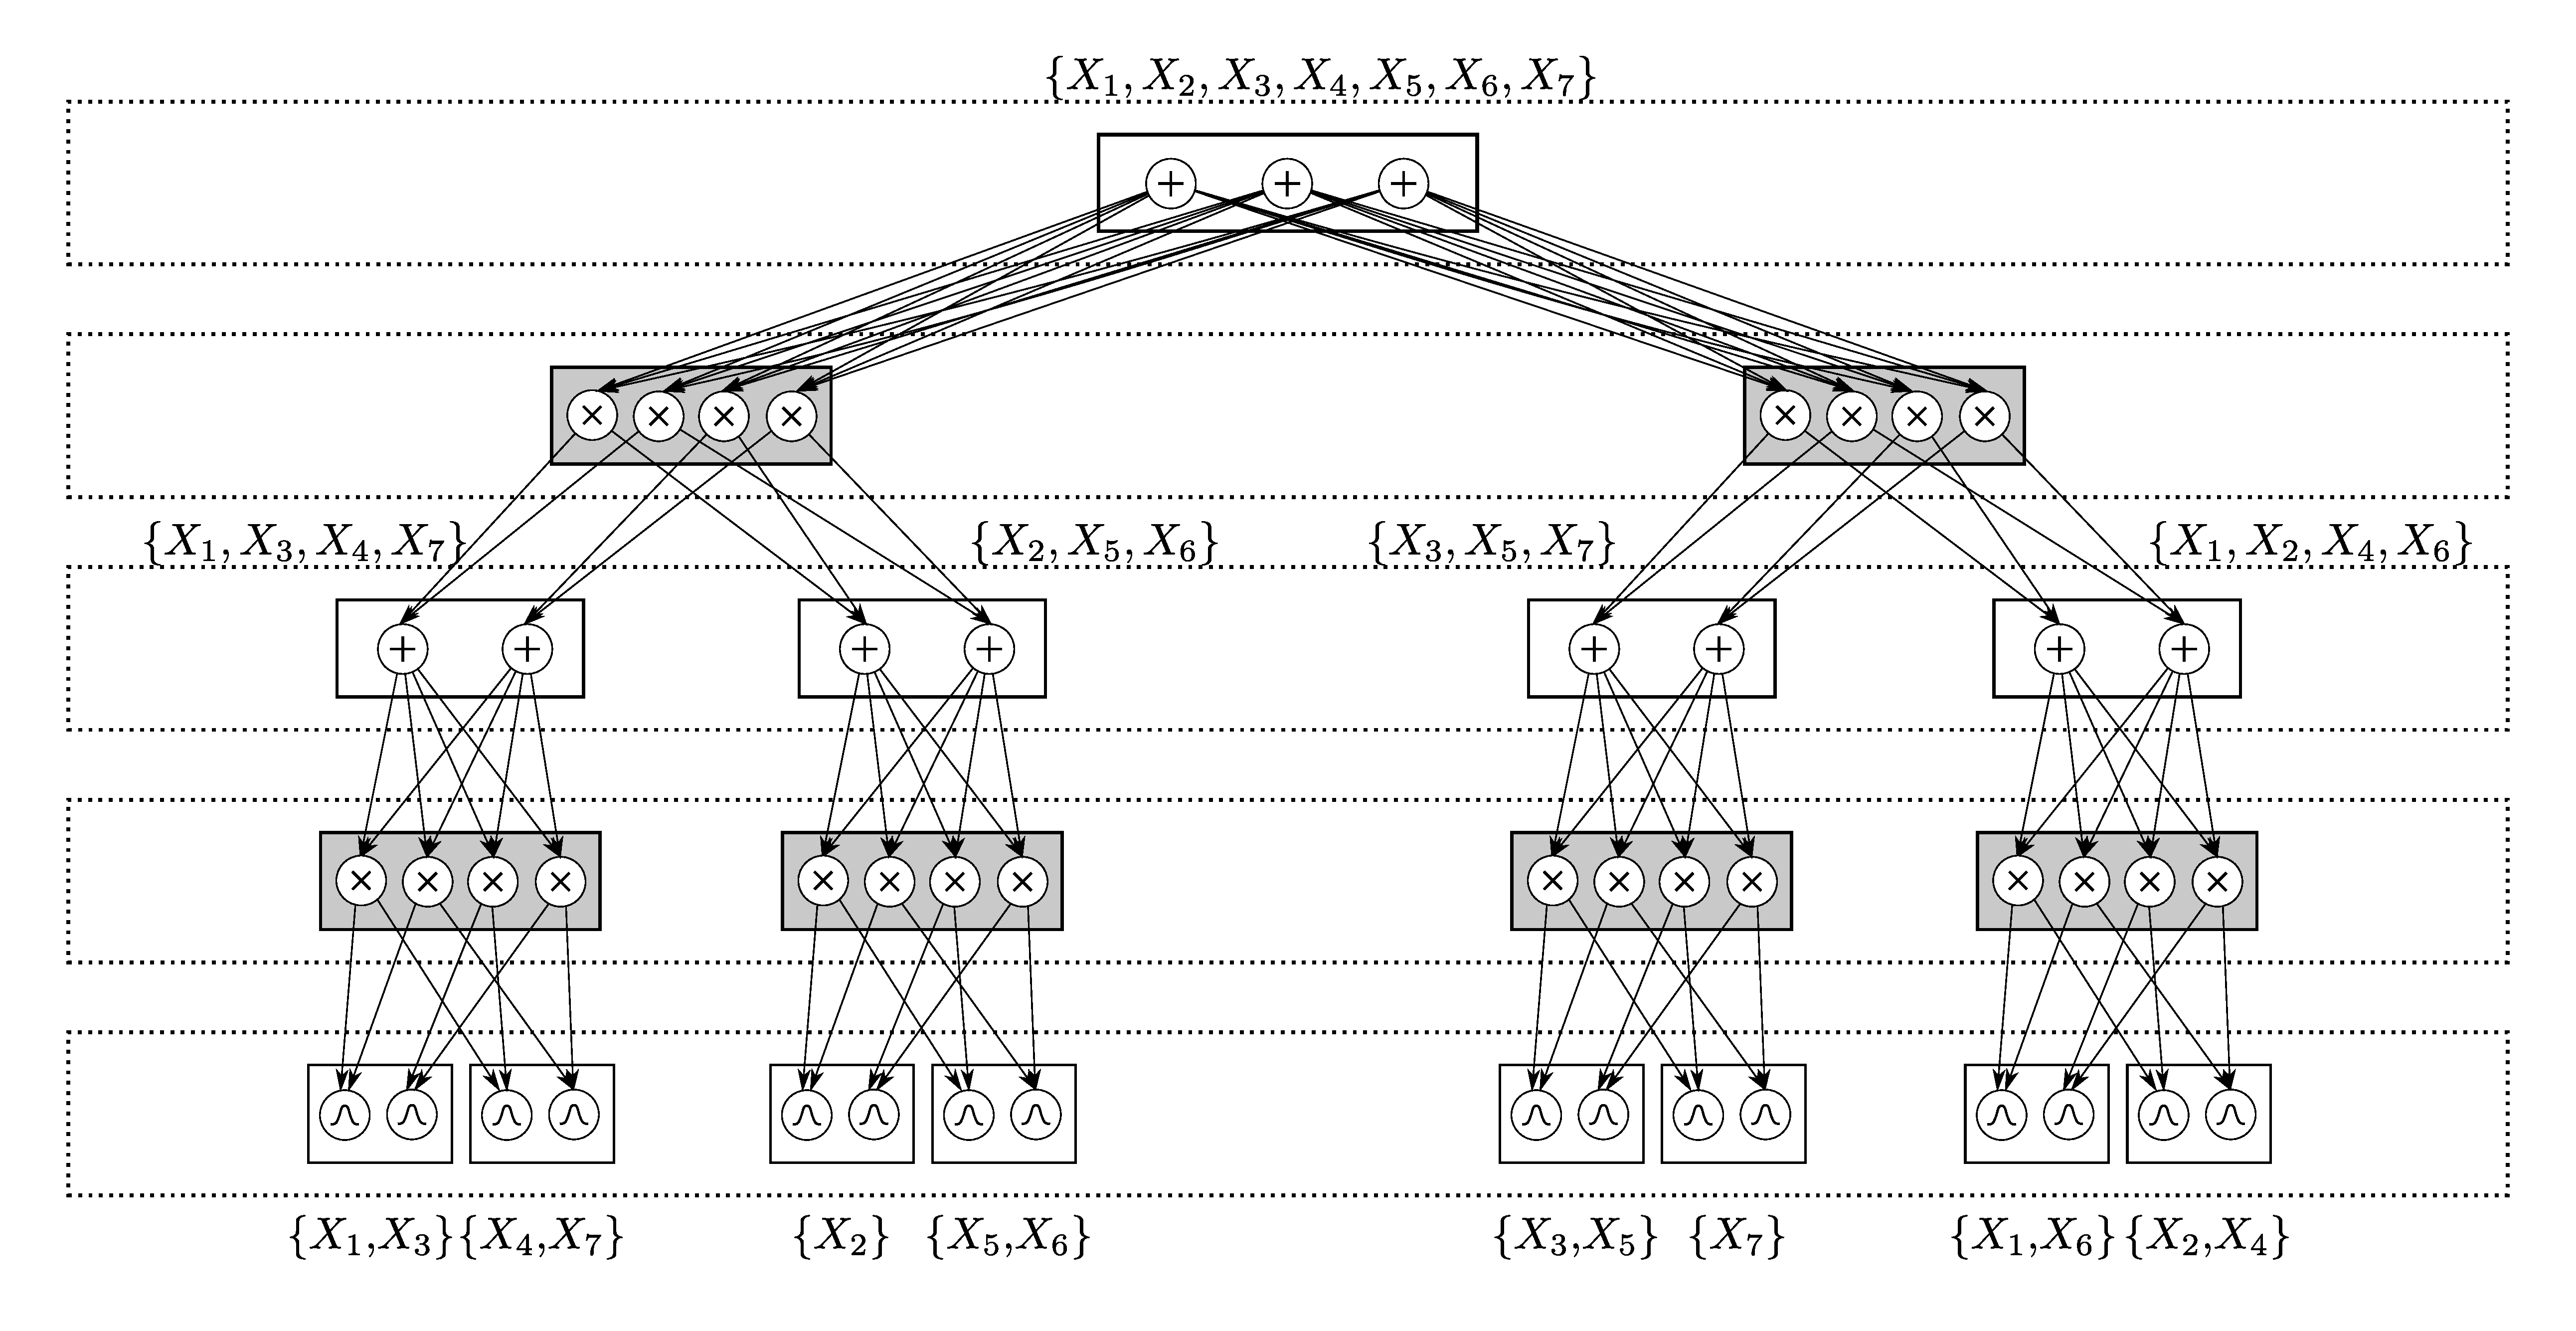
\includegraphics[width=0.8\textwidth]{example_RAT-SPN-eps-converted-to}
    \end{figure}

    \pause

    \begin{figure}
    \centering
    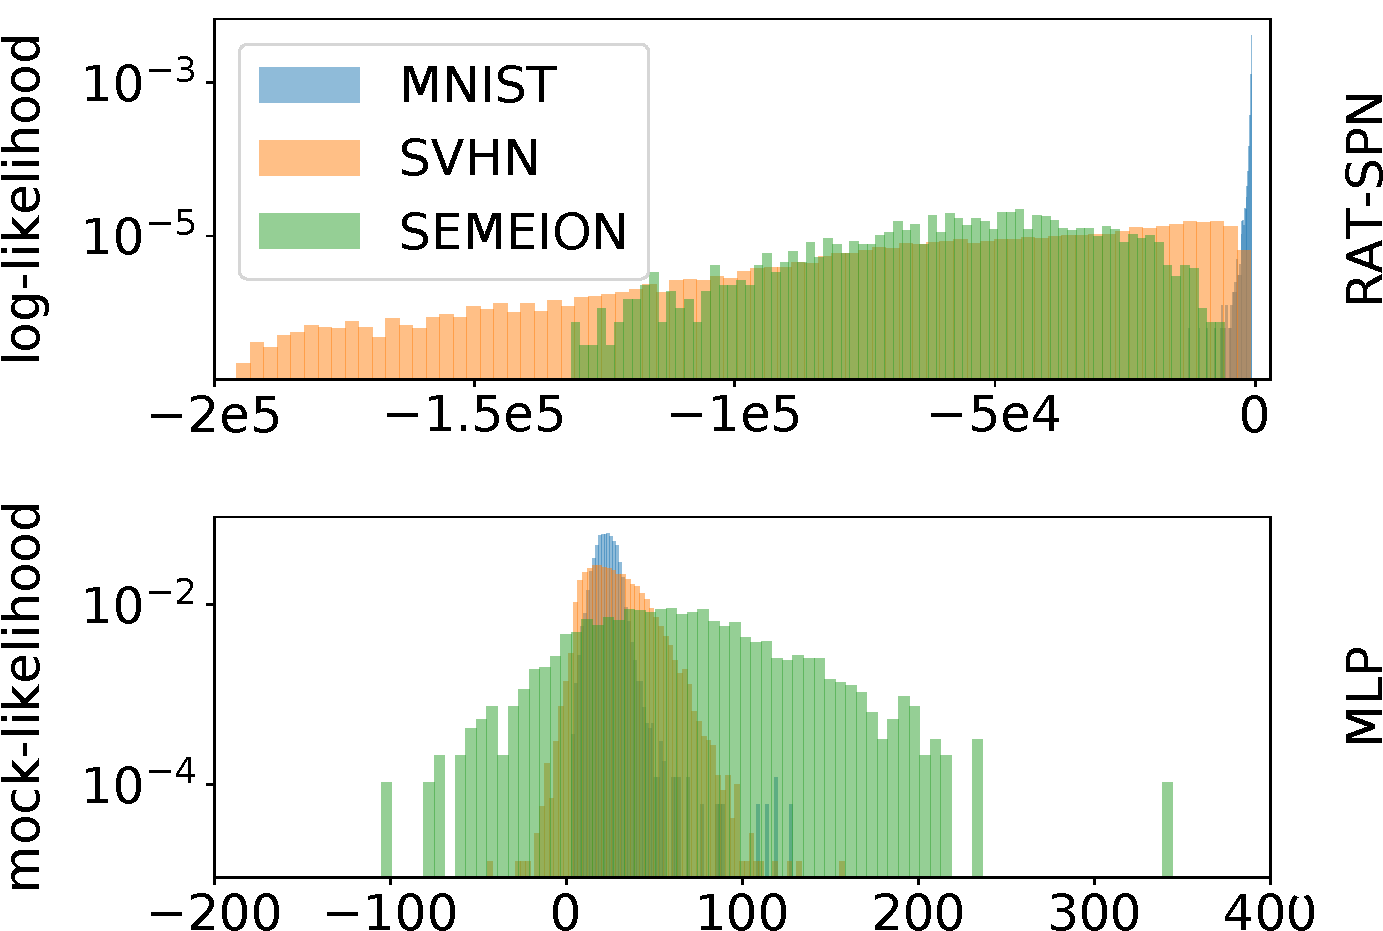
\includegraphics[width=0.6\textwidth]{transfer-testing-lambda-0-2-crop}
\end{figure}

\end{frame}

%\begin{frame}{Bayesian Structure \& Parameter Learning \small $[$Trapp2019$]$}
%  \begin{itemize}
%    \item For Bayesian structure \& parameter learning of SPNs we assume $\graph$ is a tree-shaped region graph.
%    \pause
%    \item A region graph $\rg$ is a vectorised representation of SPNs and is a connected DAG containing two types of nodes: regions ($\region \in \regions$) and partitions ($\partition \in \partitions$).
%  \end{itemize}
%  \pause
%  \begin{figure}
%  \centering
%  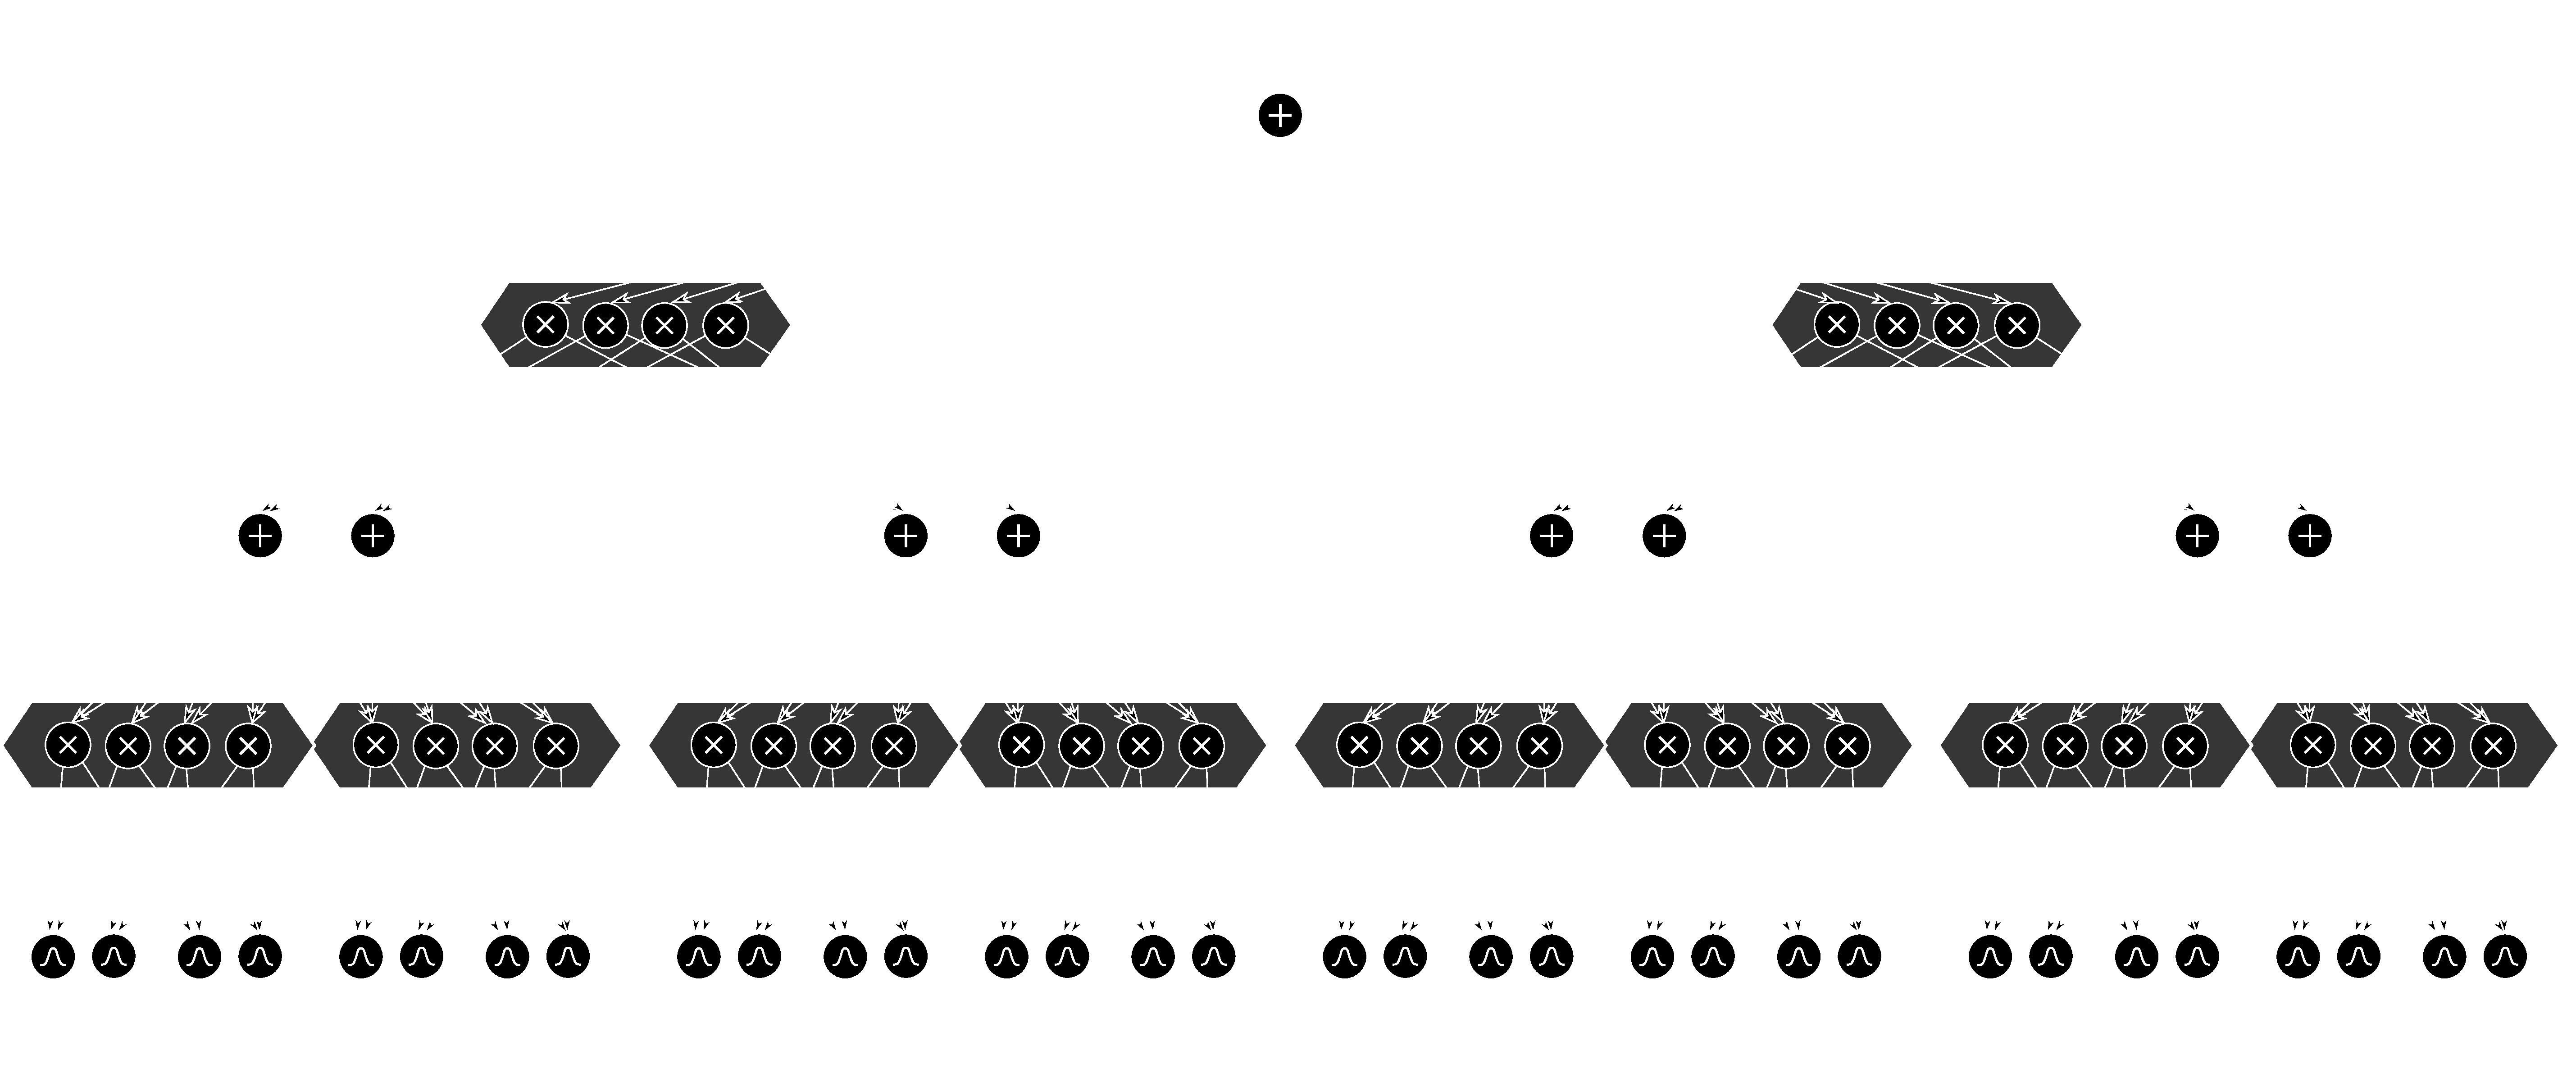
\includegraphics[width=0.9\linewidth]{region-graph}
%  \caption{Example region-graph. Based on the illustration by [Peharz2019].}
%\end{figure}
%
%\end{frame}

\begin{frame}{Bayesian Structure}
\begin{block}{Why care about Bayesian structure learning?}
\begin{itemize}
        \item Occam's razor effect prevents overfitting.
        \item Works on discrete, continuous and heterogeneous data domains.
        \item We can use nonparametric formulations, e.g.~infinite SPNs, for continual learning.
        \item Structures can be inferred even in cases of missing values using exact marginalisation.
    \end{itemize}
\end{block}
\end{frame}

\begin{frame}{Bayesian Structure}
%\begin{itemize}
%    \item We assume $\graph$ is a tree-shaped region graph, i.e., the SPN is a \emph{not} a tree.
%    \item For each dimension $d$ we introduce a latent variable $Y_{\partition,d}$ at each partition node (bucket of product nodes).
%    \item The latent variables represent an assign of $d$ to a child, given a unique path leading to the node.
%\end{itemize}
Generative model for Bayesian learning of SPNs.
\begin{figure}
    \centering
    \begin{tikzpicture}
        \node[obs] (x) {$\xnd$};
        \node[latent, left=of x] (z) {$z_{\SumNode,n}$};
        \node[latent, right=of x] (y) {$y_{\partition,d}$};
        \node[latent, below=of y] (t) {$\theta_{\Leaf,d}$};
        \node[latent, below=of z] (w) {$w_{\SumNode}$};
        \node[latent, right=of y] (o) {$\vp_{\partition}$};

        \edge {z,t} {x} ; %
        \edge {y} {x} ; %
        \edge {w} {z} ; %
        \edge {o} {y} ; %

        \plate {zs} {(z)(w)} {$\forall \SumNode \in \SumNodes$} ;
        \plate {yo} {(y)(o)} {$\forall \partition \in \partitions$} ;
        \plate {t} {(t)} {$\forall \Leaf \in \Leaves$} ;
        \plate [inner xsep=0.3cm] {xyt} {(x)(y)(t)} {$d\!\in\!1\!:\!D$} ;
        \plate [inner xsep=0.3cm] {xz} {(x)(z)(xyt.north west)} {$n\!\in\!1\!:\!N$} ;
    \end{tikzpicture}
    %\caption{Generative model for Bayesian structure learning.}\label{fig:BSPN}
\end{figure}
\end{frame}

\begin{frame}{Bayesian Structure}
Posterior inference using ancestral sampling within Gibbs.

\begin{figure}
    \centering
    \begin{tikzpicture}
        \node[obs] (x) {$\xnd$};
        \node[gray, latent, draw=gray, left=of x] (z) {$z_{\SumNode,n}$};
        \node[blue, latent, draw=blue, right=of x] (y) {$y_{\partition,d}$};
        \node[violet, latent, draw=violet, below=of y] (t) {$\theta_{\Leaf,d}$};
        \node[violet, latent, draw=violet, below=of z] (w) {$w_{\SumNode}$};
        \node[gray, latent, draw=gray, right=of y] (o) {$\vp_{\partition}$};

        \edge {z,t} {x} ; %
        \edge {y} {x} ; %
        \edge {w} {z} ; %
        \edge {o} {y} ; %

        \plate {zs} {(z)(w)} {$\forall \SumNode \in \SumNodes$} ;
        \plate {yo} {(y)(o)} {$\forall \partition \in \partitions$} ;
        \plate {t} {(t)} {$\forall \Leaf \in \Leaves$} ;
        \plate [inner xsep=0.3cm] {xyt} {(x)(y)(t)} {$d\!\in\!1\!:\!D$} ;
        \plate [inner xsep=0.3cm] {xz} {(x)(z)(xyt.north west)} {$n\!\in\!1\!:\!N$} ;
    \end{tikzpicture}
    %\caption{Generative model for Bayesian structure and learning.}\label{fig:BSPN}
\end{figure}
\end{frame}

\tikzset{
    invisible/.style={opacity=0},
    visible on/.style={alt={#1{}{invisible}}},
    alt/.code args={<#1>#2#3}{%
      \alt<#1>{\pgfkeysalso{#2}}{\pgfkeysalso{#3}} % \pgfkeysalso doesn't change the path
    },
  }


\begin{frame}{Bayesian Structure - Missing Values Experiment}
Performance under increasing amount of missing values.

\begin{figure}
\begin{center}
    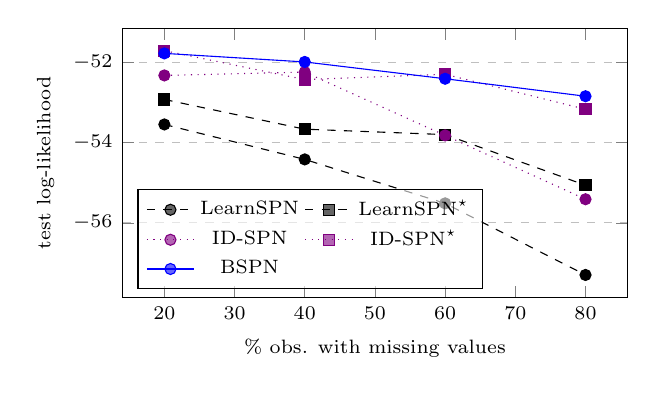
\begin{tikzpicture}
%
\begin{axis}[
%
    width=8cm,
%
    height=5cm,
%
    xlabel={\scriptsize{\% obs. with missing values}},
%
    ylabel={\scriptsize{test log-likelihood}},
%
    legend pos=south west,
    legend columns=2,
    legend style={font=\scriptsize},
    legend image post style={scale=1},
    legend style={fill opacity=0.6, draw opacity=1,text opacity=1},
    label style={font=\scriptsize},
    tick label style={font=\scriptsize},
%
    ymajorgrids=true,
%
    grid style=dashed
]

\addplot [color=black, dashed, mark=*, mark options={solid},visible on=<1->] coordinates {
    (20, -53.551654150378006)
%
    (40, -54.421205612626615)
%
    (60, -55.51437111821264)
%
    (80, -57.29533673640321)
%
    };
%
\addlegendentry{LearnSPN}

%
\addplot [color=black, dashed, mark=square*, mark options={solid},visible on=<2->] coordinates {
    (20, -52.9306308300396)
%
    (40, -53.669159658525054)
%
    (60, -53.804286870223166)
%
    (80, -55.06448194755978)
%
    };
%
\addlegendentry{LearnSPN$^\star$}
%

\addplot [color=violet, dotted, mark=*, mark options={solid},visible on=<1->] coordinates {
    (20, -52.332443930626056)
%
    (40, -52.24919890693739)
%
    (60, -53.824333727580374)
%
    (80, -55.41192445685279)
%
    };
%
\addlegendentry{ID-SPN}

%
\addplot [color=violet, dotted, mark=square*, mark options={solid},visible on=<2->] coordinates {
    (20, -51.71630289170897)
%
    (40, -52.4355408358714)
%
    (60, -52.30368237732657)
%
    (80, -53.173612370558374)
%
    };
%
\addlegendentry{ID-SPN$^\star$}

\addplot [color=blue, solid, mark=*, mark options={solid}, visible on=<3->] coordinates {
    (20, -51.784)
%
    (40, -51.997)
%
    (60, -52.415)
%
    (80, -52.85)
%
    };
%
\addlegendentry{BSPN}

%
\end{axis}
%
\end{tikzpicture}
\end{center}
\caption{Results on EachMovie (D: 500, N: 5526) dataset.}
\end{figure}


\end{frame}


%
%\begin{frame}{Experiments (missing data)}
%\begin{figure}
%  \begin{minipage}{.48\textwidth}
%     \begin{tikzpicture}
%
%\begin{axis}[
%
%    width=5.5cm,
%
%    height=4cm,
%
%    xlabel={\scriptsize{\% obs. with missing values}},
%
%    ylabel={\scriptsize{test log-likelihood}},
%
%    legend pos=south west,
%    legend columns=2,
%    legend style={font=\tiny},
%    legend image post style={scale=0.5},
%    legend style={fill=background, draw=white, fill opacity=0.6, draw opacity=1,text opacity=1},
%    label style={font=\tiny},
%    tick label style={font=\tiny},
%
%    ymajorgrids=true,
%
%    grid style=dashed,
%
%    cycle list name=my black white
%
%]
%
%\addplot coordinates {
%
%    (20, -53.551654150378006)
%
%    (40, -54.421205612626615)
%
%    (60, -55.51437111821264)
%
%    (80, -57.29533673640321)
%
%    };
%
%\addlegendentry{LearnSPN}
%
%
%\addplot coordinates {
%
%    (20, -52.9306308300396)
%
%    (40, -53.669159658525054)
%
%    (60, -53.804286870223166)
%
%    (80, -55.06448194755978)
%
%    };
%
%\addlegendentry{LearnSPN$^\star$}
%
%
%
%\addplot coordinates {
%
%    (20, -52.332443930626056)
%
%    (40, -52.24919890693739)
%
%    (60, -53.824333727580374)
%
%    (80, -55.41192445685279)
%
%    };
%
%\addlegendentry{ID-SPN}
%
%
%\addplot coordinates {
%
%    (20, -51.71630289170897)
%
%    (40, -52.4355408358714)
%
%    (60, -52.30368237732657)
%
%    (80, -53.173612370558374)
%
%    };
%
%\addlegendentry{ID-SPN$^\star$}
%
%\addplot coordinates {
%
%    (20, -51.784)
%
%    (40, -51.997)
%
%    (60, -52.415)
%
%    (80, -52.85)
%
%    };
%
%\addlegendentry{BSPN}
%
%
%\end{axis}
%
%\end{tikzpicture}
%\caption{EachMovie (D: 500, N: 5526)}
%\end{minipage}
%\begin{minipage}{.48\textwidth}
%  \begin{tikzpicture}
%
%\begin{axis}[
%
%    width=5.5cm,
%
%    height=4cm,
%
%    xlabel={\scriptsize{\% obs. with missing values}},
%
%    legend pos=north east,
%
%    ymajorgrids=true,
%
%    grid style=dashed,
%    label style={font=\tiny},
%    tick label style={font=\tiny},
%
%    cycle list name=my black white,
%
%]
%
%\addplot coordinates {
%
%    (20, -161.41130223478262)
%
%    (40, -163.56351684466114)
%
%    (60, -162.96930286251663)
%
%    (80, -168.00941901059738)
%
%    };
%
%\addlegendentry{learnSPN}
%
%
%
%
%\addplot coordinates {
%
%    (20, -161.4285603783307)
%
%    (40, -165.36322925292424)
%
%    (60, -164.87160515320465)
%
%    (80, -164.53405856701238)
%
%    };
%
%\addlegendentry{learnSPN$^\star$}
%
%
%
%\addplot coordinates {
%
%    (20, -152.1845925143198)
%
%    (40, -154.95268171360382)
%
%    (60, -158.58576871121716)
%
%    (80, -165.45426630310263)
%
%    };
%
%\addlegendentry{ID-SPN}
%
%
%\addplot coordinates {
%
%    (20, -152.26143497732696)
%
%    (40, -153.5671636300716)
%
%    (60, -153.5671636300716)
%
%    (80, -157.2684578353222)
%
%    };
%
%\addlegendentry{ID-SPN$^\star$}
%
%\addplot coordinates {
%
%    (20, -157.078)
%
%    (40, -157.876)
%
%    (60, -158.625)
%
%    (80, -159.123)
%
%    };
%
%\addlegendentry{BSPN}
%  \legend{}; % empty the legend so as not to print it
%
%\end{axis}
%
%\end{tikzpicture}
%\caption{WebKB (D: 839, N: 3361)}
%\end{minipage}
%\begin{minipage}{.5\textwidth}
%  \begin{tikzpicture}
%
%\begin{axis}[
%
%    width=5.5cm,
%
%    height=4cm,
%
%    xlabel={\scriptsize{\% obs. with missing values}},
%
%    legend pos=north east,
%
%    ymajorgrids=true,
%
%    grid style=dashed,
%    label style={font=\tiny},
%    tick label style={font=\tiny},
%
%    cycle list name=my black white
%
%]
% 
%
%\addplot coordinates {
%
%    (20, -250.83622675798426)
%
%    (40, -261.1124401206212)
%
%    (60, -266.0005946312015)
%
%    (80, -273.39617177834293)
%
%    };
%
%\addlegendentry{learnSPN}
%
%
%
%\addplot coordinates {
%
%    (20, -284.24099564475125)
%
%    (40, -261.6701870807035)
%
%    (60, -265.4755544697035)
%
%    (80, -297.06332858812755)
%
%    };
%
%\addlegendentry{learnSPN$^\star$}
%
%
%
%\addplot coordinates {
%
%    (20, -250.68554855757577)
%
%    (40, -253.81061585454546)
%
%    (60, -261.81913693030305)
%
%    (80, -272.27580261212125)
%
%    };
%
%\addlegendentry{ID-SPN}
%
%
%
%\addplot coordinates {
%
%    (20, -249.82204944242426)
%
%    (40, -252.33469486666664)
%
%    (60, -254.56216942424243)
%
%    (80, -256.8125317606061)
%
%    };
%
%\addlegendentry{ID-SPN$^\star$}
%
%\addplot coordinates {
%
%    (20, -251.551)
%
%    (40, -254.101)
%
%    (60, -255.551)
%
%    (80, -256.144)
%
%    };
%
%\addlegendentry{BSPN}
%  \legend{}; % empty the legend so as not to print it
%
%\end{axis}
%
%\end{tikzpicture}
%\caption{BBC (D: 1058, N: 1895)}
%\end{minipage}
%\end{figure}
%
%\end{frame}
